\documentclass[../main.tex]{subfiles}

\begin{document}

\ifSubfilesClassLoaded{\setcounter{numpractica}{10}}{}


\practica{Sistema Operativo en Tiempo Real (RTOS)}

    \subsection{Objetivos}
        \begin{itemize}
            \item Integrar un sistema operativo en tiempo real en un procesador con capacidad expropiativa.
            \item Entender cómo se interconexionan los diferentes módulos del RTOS para lograr su funcionalidad.
        \end{itemize}

    \subsection{Fundamentos teóricos}

        Un \textbf{Sistema Operativo en Tiempo Real} o \textbf{RTOS} (\textit{Real-Time Operating System}) es un software diseñado para administrar los recursos del microprocesador y garantizar que las diferentes tareas que pueda realizar, se ejecuten en tiempos predecibles. 

        En un entorno \textit{bare-metal} estándar, la temporización depende de retardos con espera activa o interrupciones de temporizadores, pero al no existir un supervisor, existe mayor posibilidad de fallos, o tareas que se atascan y bloquean al resto, al contar habitualmente con multitarea cooperativa y no expropiativa.

        Un RTOS añade una capa superior de gestión, donde se divide el tiempo en trozos (\textit{time-slicing}) y se va dando a cada tarea según lo necesite, siendo capaz, mediante configuración de prioridades, de ejecutar ciertas tareas en momentos concretos (por ejemplo, para sistemas temporizados críticos como vehículos o maquinaria industrial).

        \subsubsection{Arquitectura y Planificación Expropiativa en Cortex-M}

            En esta práctica se utiliza un RTOS de tipo expropiativo sobre la arquitectura ARM Cortex-M7 de nuestro \MCU. El kernel puede suspender la ejecución de una tarea en curso y ceder el procesador a otra tarea de mayor prioridad o a la que le corresponda el siguiente turno de ejecución en caso de empate de prioridades.

            La interacción entre el hardware del microprocesador y el núcleo del RTOS se realiza mediante tres interrupciones del Cortex-M:

            \begin{itemize}
                \item \textbf{SysTick} Generará las interrupciones periódicas que indicarán el cambio de contexto entre las diferentes tareas en ejecución del sistema.
                \item \textbf{SVC (Supervisor Call):} Es una excepción provocada por software mediante la instrucción assembly \texttt{svc 0}. Se utiliza durante la fase de arranque para realizar la transición inicial del modo privilegiado del procesador al modo de ejecución de la primera tarea del RTOS (\texttt{vTaskStartScheduler}).
                \item \textbf{PendSV (Pendable Service Call):} Es una excepción que se configura con la prioridad de hardware \textbf{más baja posible} en el NVIC. La función de \texttt{PendSV} es ejecutar el cambio de contexto (\textit{context switch}). Al tener la menor prioridad, se garantiza que cualquier interrupción de periféricos (\PER{UART}, \PER{GPIO}, \PER{TIMx}) finalice antes de que el RTOS intervenga.
            \end{itemize}

        \subsubsection{Bloque de Control de Tarea (TCB) y Estructuras Internas}

            Para gestionar la ejecución multitarea, el kernel del RTOS asocia a cada tarea una estructura llamada \textbf{TCB} (\textit{Task Control Block}). El TCB contiene los datos necesarios sobre la tarea como para que el RTOS sea capaz de retirarla de ejecución o reanudarla cuando el planificador así lo dictamine.

            \begin{itemize}
                \item Puntero a la Cima de Pila (\texttt{pxTopOfStack}): Apunta a la posición actual del puntero de pila de la tarea. Al ejecutarse un cambio de contexto, los registros de la CPU ($R0$-$R12$, $LR$, $PC$, $xPSR$) se guardan en esta pila y se actualiza este puntero. Así se preserva el estado actual
                \item Punteros a las listas internas del kernel bloqueadas o suspendidas para vincular directamente la tarea a una de ellas.
                \item Prioridad de la Tarea (\texttt{uxPriority}): Determina el nivel de preferencia de ejecución asignado a la tarea. Cuanta más prioridad tenga, más veces entrará en ejecución, aunque en última instancia esto depende de la política de planificación.
                \item Límite de la Pila (\texttt{pxStack}): Puntero a la base de la pila utilizada opcionalmente para detectar desbordamientos (\textit{stack overflow}).
            \end{itemize}

            El kernel mantiene internamente varias listas enlazadas ordenadas por prioridad. Cuando la interrupción periódica \texttt{xPortSysTickHandler} (\texttt{Systick\_Handler}) se ejecuta, el planificador consulta la lista de tareas bloqueadas y la lista de tareas listas. La función \texttt{vTaskSwitchContext} simplemente localiza el TCB de mayor prioridad disponible y actualiza el puntero \texttt{pxCurrentTCB}.

        \subsubsection{Gestión de Memoria: Pila (Stack) y Memoria Dinámica (Heap)}

            En un sistema \textit{bare-metal} existe un único espacio de pila (\textit{Main Stack Pointer} o \textbf{MSP}) utilizado por todo el código y por las interrupciones. En un RTOS, con la introducción de las tareas, la estructura se complica como puede verse en la \Cref{fig:memory_layout}.

            \begin{itemize}
                \item \textbf{MSP (Main Stack Pointer):} Se utiliza durante la fase de arranque, y la gestión del RTOS (planificador y cambio de contexto), así como para atender la ejecución de los manejadores de interrupción (ISRs). Esto último es especialmente interesante pues así no es necesario que cada tarea reserve espacio en la pila para todas las posibles interrupciones que sufra.
                \item \textbf{PSP (Process Stack Pointer):} Cada tarea creada dispone de su propio espacio de pila independiente en la memoria RAM, al que el hardware conmuta automáticamente cuando la tarea entra en estado \textit{Running}.
                \item \textbf{Gestión de Heap:} FreeRTOS reserva una región contigua en la sección \texttt{.bss} de la RAM. Al crear una tarea, el kernel asigna automáticamente en este heap la memoria necesaria tanto para el TCB como para la pila privada de la tarea. 
            \end{itemize}

            \begin{figure}[htbp]
                \centering
                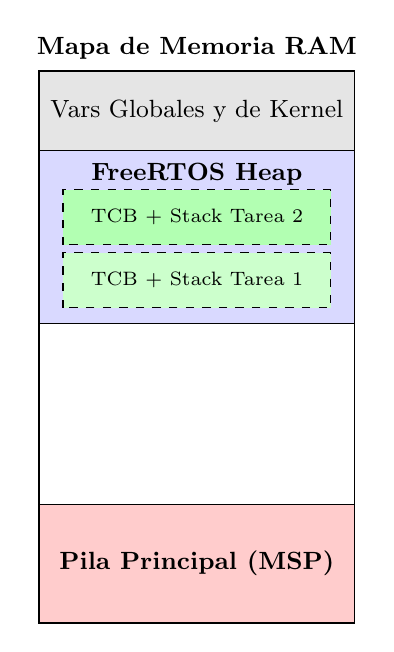
\begin{tikzpicture}[node distance=0cm, >=stealth, font=\small]
                    % Contenedor principal de RAM
                    \draw[thick] (0,0) rectangle (4,7);
                    \node at (2,7.3) {\textbf{Mapa de Memoria RAM}};

                    % Secciones
                    \draw[fill=gray!20] (0,6) rectangle (4,7);
                    \node at (2,6.5) {Vars Globales y de Kernel};

                    \draw[fill=blue!15] (0,3.8) rectangle (4,6);
                    \node at (2,5.7) {\textbf{FreeRTOS Heap}};
                    
                    % TCBs y Stacks dentro del Heap
                    \draw[fill=green!20, dashed] (0.3,4.0) rectangle (3.7,4.7);
                    \node at (2,4.35) {\scriptsize TCB + Stack Tarea 1};

                    \draw[fill=green!30, dashed] (0.3,4.8) rectangle (3.7,5.5);
                    \node at (2,5.15) {\scriptsize TCB + Stack Tarea 2};

                    \draw[fill=white!20] (0,1.5) rectangle (4,3.8);

                    \draw[fill=red!20] (0,0) rectangle (4,1.5);
                    \node at (2,0.75) {\textbf{Pila Principal (MSP)}};

                \end{tikzpicture}
                \caption{Disposición de la memoria RAM: separación entre el MSP (utilizado por las interrupciones) y las pilas independientes de cada tarea (PSP) alojadas en el Heap de FreeRTOS.}
                \label{fig:memory_layout}
            \end{figure}

        \subsubsection{Diagrama de Interacción entre Interrupciones y Tareas}

            La Figura~\ref{fig:rtos_execution_flow} ilustra el flujo temporal de interacción entre el temporizador de sistema, las tareas de usuario y el mecanismo de cambio de contexto de FreeRTOS.

            \begin{figure}[htbp]
                \centering
                \begin{tikzpicture}[node distance=1.5cm, >=stealth, font=\small]
                    % Estilos de bloques
                    \tikzstyle{hw} = [draw, fill=red!10, minimum width=2.5cm, minimum height=0.8cm, align=center, rounded corners=2pt]
                    \tikzstyle{kernel} = [draw, fill=blue!10, minimum width=2.5cm, minimum height=0.8cm, align=center, rounded corners=2pt]
                    \tikzstyle{task} = [draw, fill=green!10, minimum width=2.5cm, minimum height=0.8cm, align=center, rounded corners=2pt]
                    \tikzstyle{line} = [draw, ->, thick]
                    \tikzstyle{dashedline} = [draw, ->, thick, dashed]

                    % Nodos
                    % Arranque / SVC
                    \node [hw] (svc) {\textbf{SVC ISR}\\(\texttt{svc 0} en startup)};
                    \node [kernel, right=1.8cm of svc] (svc_handler) {\textbf{vPortSVCHandler}\\Inicializa TCBs y listas\\Lanza primera tarea};

                    % SysTick y flujo continuo
                    \node [hw, below=1.5cm of svc] (systick) {\textbf{SysTick ISR}\\(Hardware Timer)};
                    \node [kernel, right=1.8cm of systick] (tick_handler) {\textbf{xPortSysTickHandler}\\Actualiza \texttt{xTickCount}\\Lee estructuras TCB\\Elige siguiente tarea};
                    
                    % PendSV y Cambio de Contexto
                    \node [kernel, below=1.2cm of tick_handler] (pendsv) {\textbf{xPortPendSVHandler}\\Solicitado (Pending)};
                    \node [kernel, below=1.2cm of pendsv] (switch) {\textbf{vTaskSwitchContext}\\Guarda contexto Tarea A\\Carga contexto Tarea B};
                    
                    % Tareas
                    \node [task, below right=1.2cm and 0.6cm of switch] (taskB) {\textbf{Tarea B (Alta Prioridad)}\\Pasa a estado \textit{Running}};
                    \node [task, below left=1.2cm and 0.6cm of switch] (taskA) {\textbf{Tarea A (Baja Prioridad)}\\Suspendida/Bloqueada};

                    % Conexiones
                    % Arranque
                    \path [line] (svc) -- node[above] {Al inicio} (svc_handler);
                    \path [dashedline] (svc_handler) -- node[left] {Prepara TCBs} (tick_handler);

                    % Bucle Periódico
                    \path [line] (systick) -- node[above] {Cada tick} (tick_handler);
                    \path [line] (tick_handler) -- node[left] {Dispara PendSV} (pendsv);
                    \path [line] (pendsv) -- node[left] {Ejecuta al terminar otras ISRs} (switch);
                    \path [line] (switch) |- (taskB);
                    \path [line] (switch) |- (taskA);

                \end{tikzpicture}
                \caption{Flujo completo de ejecución: arranque mediante excepción SVC, inspección de estructuras TCB en SysTick y cambio de contexto diferido con PendSV.}
                \label{fig:rtos_execution_flow}
            \end{figure}

    \subsection{Desarrollo de la práctica}

        El primer paso es descargarse el paquete completo de FreeRTOS. Para ello descargamos el siguiente repositorio:

        \begin{lstlisting}
            > git clone https://github.com/FreeRTOS/FreeRTOS-LTS/
        \end{lstlisting}

        Y nos aseguramos de estar en la rama \texttt{202604-LTS} (es con la que se han hecho las pruebas, si hay una más nueva puedes probar también, pero quizá cambien detalles de la configuración).

        \begin{lstlisting}
            > cd FreeRTOS-LTS 
            > git checkout 202604-LTS 
        \end{lstlisting}

        El repositorio es bastante extenso, pero a nosotros nos interesan unos archivos muy concretos, marcados en rojo en el siguiente diagrama. Echa un vistazo en el interior para mirar, a vista de pájaro, los contenidos de cada uno. Normalmente, la selección de qué ficheros se utilizan se hace desde archivos de configuración globales, pero nosotros lo vamos a hacer a mano por simplicidad.
        
        \definecolor{doccomment}{rgb}{0.4, 0.8, 0.4}
        \definecolor{filecolor}{rgb}{0.70,0.00,0.00}
        \newcommand{\grcomment}[1]{\DTcomment{\textcolor{doccomment}{-- #1}}}
        \newcommand{\colorfile}[1]{\textcolor{filecolor}{#1}}

        \dirtree{%
            .1 FreeRTOS-Kernel/\grcomment{Código fuente de las prácticas}.
                .2 \colorfile{list.c}\grcomment{Código fuente de lista enlazada}.
                .2 \colorfile{queue.c}\grcomment{Código fuente de cola}.
                .2 \colorfile{tasks.c}\grcomment{Código fuente de gestión de tareas}.
                .2 \colorfile{timers.c}\grcomment{Código fuente de gestión de timers}.
                .2 examples/\grcomment{Ejemplo de uso de FreeRTOS}.
                    .3 cmake\_example/\grcomment{Ejemplo de aplicación}.
                        .4 \colorfile{main.c}/\grcomment{Archivo de aplicación}.
                    .3 template\_configuration/\grcomment{Ejemplo de configuración}.
                        .4 \colorfile{FreeRTOSConfig.h}/\grcomment{Archivo de configuración}.
                .2 include/\grcomment{Cabeceras de los diferentes componentes de FreeRTOS}.
                    .3 \colorfile{deprecated\_definitions.h}\grcomment{Definiciones en desuso}.
                    .3 \colorfile{FreeRTOS.h}\grcomment{Definiciones de macros, funciones y estructuras utilizadas}.
                    .3 \colorfile{list.h}\grcomment{Cabecera de lista enlazada}.
                    .3 \colorfile{mpu\_wrappers.h}\grcomment{Cabecera utlizada con unidad de protección de memoria}.
                    .3 \colorfile{portable.h}\grcomment{Cabecera para incluir los ports de procesador específicos}.
                    .3 \colorfile{projdefs.h}\grcomment{Definiciones genéricas de tipos y errores}.
                    .3 \colorfile{queue.h}\grcomment{Cabecera de cola}.
                    .3 \colorfile{stack\_macros.h}\grcomment{Cabecera para controlar el stack overflow opcionalmente}.
                    .3 \colorfile{task.h}\grcomment{Cabecera para gestión de tareas}.
                    .3 \colorfile{timers.h}\grcomment{Cabecera para gestión de timers}.
                .2 portable/\grcomment{Código específico de los diferentes procesadores soportados}.
                    .3 GCC/\grcomment{Código para compiladores GCC}.
                        .4 ARM\_CM7/\grcomment{Código para procesadores ARM-M7}.
                            .5 r0p1/\grcomment{Versión r0p1 del procesador}.
                                .6 \colorfile{port.c}\grcomment{Funciones específicas de procesador}.
                                .6 \colorfile{portmacro.h}\grcomment{Macros y definiciones específicas de procesador}.
                    .3 MemMang/\grcomment{Código para gestión de memoria}.
                        .4 \colorfile{heap\_4.c}\grcomment{Código fuente para gestión de memoria dinámica}.
        }

        Ahora debemos configurar todos los elementos de la práctica. En concreto, configurar FreeRTOS, hacer el puente con nuestro código y BSP, y finalmente integrarlo todo en un código main.

        El primer paso es editar el archivo \texttt{FreeRTOSConfig.h} para poner la configuración concreta de nuestro procesador. Debemos encontrar las siguientes definiciones (algunas son nuevas) y añadirlas o editarlas en el archivo:

        \begin{lstlisting}
            //1)  Para que la temporización funcione bien, debemos indicar la frecuencia 
            //    de nuestro reloj (16Mhz), y el tick rate que queremos (en este caso)
            //    lo configuramos para 1 tick cada milisegundo
            #define configCPU_CLOCK_HZ    ( ( unsigned long ) 16000000 )
            #define configTICK_RATE_HZ                         1000

            //2)  Ahora configuramos las prioridades para las interrupciones del kernel
            //    (para la planificación). No configurar esto hace que la compilación no
            //    funcione
            #define configPRIO_BITS                              4
            #define configLIBRARY_LOWEST_INTERRUPT_PRIORITY      15
            #define configLIBRARY_MAX_SYSCALL_INTERRUPT_PRIORITY  5

            #define configKERNEL_INTERRUPT_PRIORITY \
                ( configLIBRARY_LOWEST_INTERRUPT_PRIORITY << (8 - configPRIO_BITS) )

            #define configMAX_SYSCALL_INTERRUPT_PRIORITY \
                ( configLIBRARY_MAX_SYSCALL_INTERRUPT_PRIORITY << (8 - configPRIO_BITS) )

            //3)  Quitamos las comprobaciones de stack overflow pues requiere de 
            //    alguna implementación adicional
                #define configCHECK_FOR_STACK_OVERFLOW        0
        \end{lstlisting}

        Lo siguiente será puentear las interrupciones de sistema a las definidas en \texttt{port.c}. Son tres:

        \begin{enumerate}
            \item \texttt{vPortSVCHandler}: Gestiona la excepción de llamada a supervisor (en este caso el supervisor es el RTOS). Hay que hacer que se llame ante la interrupción \texttt{SVC} mapeando el manejador por defecto \texttt{SVC\_Handler}.
            \item \texttt{xPortPendSVHandler}: Gestiona la excepción de llamada pendiente para el cambio de contexto. Este tipo de interrupción tiene la menor prioridad posible, para que todas las otras interrupciones (periféricos principalmente) tengan prioridad sobre ella. Se guarda el contexto de la tarea actual en el stack, y se llama al planificador para cambiar de tarea. Hay que hacer que se llame ante la interrupción \texttt{PendSV} mapeando el manejador por defecto \texttt{PendSV\_Handler}.
            \item \texttt{xPortSysTickHandler}: Gestiona las interrupciones del ticker del sistema para que el RTOS lleve la cuenta del tiempo y pueda planificar las tareas de manera acorde. Hay que hacer que se llame ante la interrupción \texttt{SysTick} mapeando el manejador por defecto \texttt{SysTick\_Handler}.
        \end{enumerate}

        Esta configuración se debe hacer desde el archivo de inicialización \texttt{startup\_stm32f723iekx.s} con las siguientes instrucciones:

        \begin{lstlisting}
            .weak	SVC_Handler
            .thumb_set SVC_Handler,vPortSVCHandler

            .weak	PendSV_Handler
            .thumb_set PendSV_Handler,xPortPendSVHandler

            .weak	SysTick_Handler
            .thumb_set SysTick_Handler,xPortSysTickHandler
        \end{lstlisting}

        Ahora solo quedará gestionar el archivo principal \texttt{main.c}, que tendrá esta forma:

        \begin{lstlisting}
            #include "FreeRTOS.h"
            #include "task.h"
            #include "queue.h"

            #include "bsp.h"
            #include "stdio.h"

            void Task1(void *pvParameters) {
                for (;;) {
                    //... completar hacer toggle a un LED (por ejemplo PA5)
                    vTaskDelay(pdMS_TO_TICKS(500)); // Delay 500 ms
                }
            }


            void GPIO_Init(void) {
                //... completar inicializar los GPIOs que se vayan a utilizar
            }

            int main(void) {
                // 1. Initialize peripherals
                GPIO_Init();


                // 2. Create FreeRTOS Tasks
                xTaskCreate(Task1, "LED_Task1", 128, NULL, 1, NULL);
                //... completar crear más tareas que enciendan por ejemplo otros leds

                // 3. Start Scheduler (never returns)
                vTaskStartScheduler();

                while (1); // aquí no debería llegar nunca
            }
        \end{lstlisting}

        Es importante saber que no podemos (o no debemos, mejor dicho) inicializar manualmente componentes del sistema como \PER{SysTick}, ya que ahora lo maneja nuestro RTOS. También hay que tener en cuenta que se modifcarán parámetros del \PER{NVIC} automáticamente, por lo que hay que tener especial cuidado al añadir nuevas interrupciones, sin enmascarar otras.
        


    \subsection{Para hacer más}

        Los sistemas operativos en tiempo real ofrecen funciones para sincronización de tareas mediante semáforos, mutex, variables condicionales y demás mecanismos que, mediante la atomicidad, aseguran ciertos comportamientos ante condiciones de carrera. Investiga cómo se resuelve esto en RTOS, y qué opciones hay al respecto.
 
\end{document}